%!TEX root = ../document.tex
\chapter{Login Parcours}
Das nachfolgende Kapitel beschreibt den Login Parcours der Broken-Web-Applikation. Hierzu folgt eine kurze Erläuterung um was es sich bei diesem Parcours handelt. Anschließend werden die einzelnen Übungslevel vorgestellt und gezeigt wie diese zu lösen sind. Abgeschlossen wird das Kapitel mit einem kurzen Ausblick  wie der Login Parcours erweitert werden kann. 

\section{Erklärung}
Der Login Parcours umfasst eine Reihe von Rätseln, bei denen der Einsteiger versuchen muss, dass Passwort einer gegebenen Login-Maske herauszufinden. Hierzu enthält jedes Level eine kurze Beschreibung mit Hinweisen, wie das Rätsel zu lösen ist (z. B. in dem der JavaScript-Code inspiziert oder eine unverschlüsselte PCAP Datei ausgelesen werden soll). \\ 
Das Ziel des Parcours ist es das Interesse des Einsteigers zu wecken, indem er einfache Aufgabestellungen lösen muss, die dem Finden von Sicherheitslücken ähneln. Zudem soll die Denkweise in Bezug auf diese Lücken geschult und gängige Gegenstände der Themengebiete wie Verschlüsselung näher gebracht werden. Darüber hinaus soll hierbei ein Spaßfaktor entstehen, sodass die Einsteiger Lust bekommen sich genauer mit der Thematik der IT-Sicherheit zu beschäftigen. 

\section{Ablauf}
Der Einstiegspunkt zu den Aufgaben entspricht der Überblickseite (Siehe Abbildung \ref{fig:login-parcours-hauptseite}) des Login-Parcours. Dort ist jedes Level mit kurzer Überschrift bzgl. der Art des Rätsels verlinkt.

\begin{figure}[H]
	\centering
	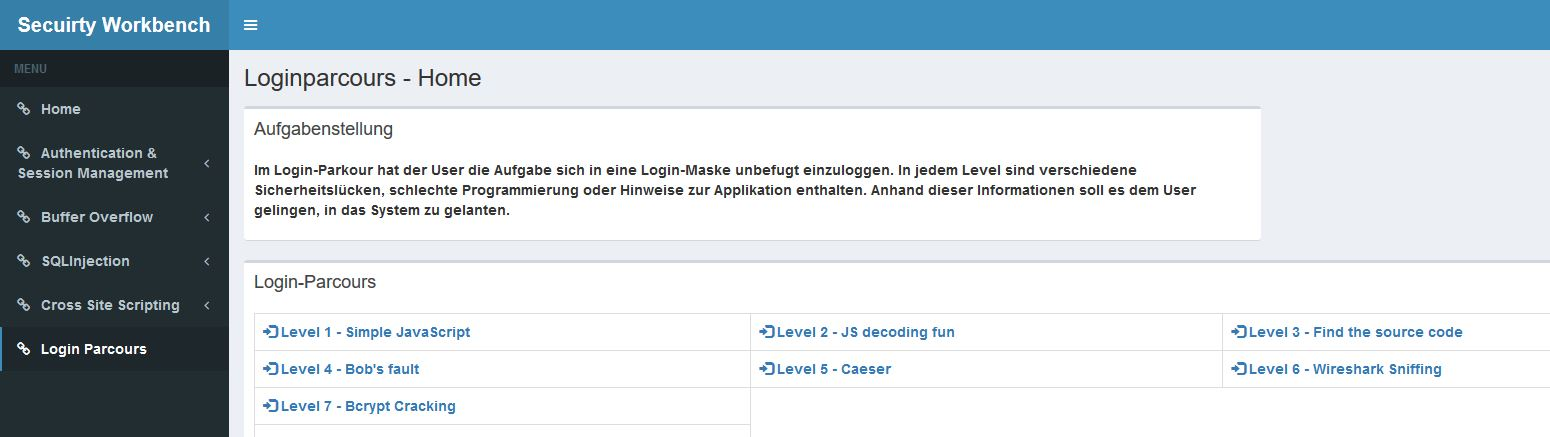
\includegraphics[width=\textwidth]{images/LoginParcours/login_parcours_hauptseite.jpg}
	\caption{Überblicksseite des Login Parcours}
	\label{fig:login-parcours-hauptseite}
\end{figure}

Der prinzipielle Ablauf jedes Rätsel ist gleich. Der Anwender bekommt einen Startbutton, mit dem eine Login-Maske erscheint. Diese ist mit einer Kurzbeschreibung ausgestattet. Wird ein Rätsel gelöst, so erscheint die dazugehörige Erfolgsmeldung und ein Verweis auf das nächste Level. 

\subsection{Level 1 - JavaScript-Code}
Im ersten Level muss der Einsteiger den JavaScript-Code auslesen, in dem fälschlicherweise die Validierung des Usernamen und Passworts enthalten ist. Der Start des Levels entspricht der Login-Maske wie in Abbildung \ref{fig:login-parcours-level1}.

\begin{figure}[H]
	\centering
	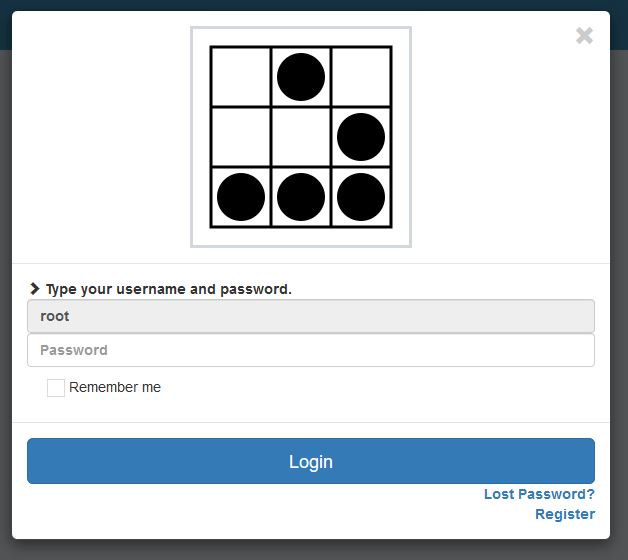
\includegraphics[width=\textwidth]{images/LoginParcours/login_level1.jpg}
	\caption{Login-Maske des ersten Levels}
	\label{fig:login-parcours-level1}
\end{figure}

Der Einsteiger soll sich mit einem Rechtsklick und \colorbox{altgray}{\lstinline|Seitenquelltext anzeigen|}, den Sourcecode anzeigen lassen. Wird dieser genauer betrachtet so wird erstichtlich, dass die Validierung des Usernamen und Passwort in einem Skript geschieht. Dort findet der Einsteiger auch das Passwort \colorbox{altgray}{\lstinline|hallo123|} zum vorgegebenen Usernamen \colorbox{altgray}{\lstinline|root|}. Abbildung \ref{fig:login-parcours-level1-solution} zeigt den zugehörigen Codeausschnitt. 

\begin{figure}[H]
	\centering
	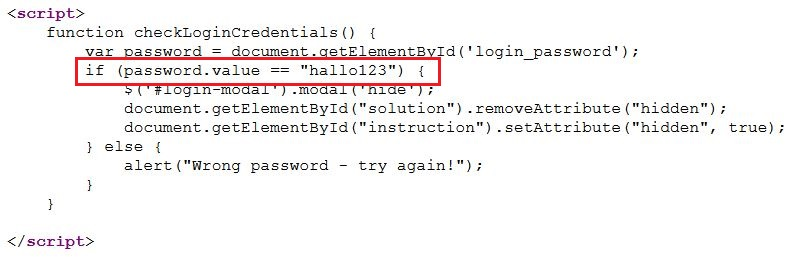
\includegraphics[width=\textwidth]{images/LoginParcours/login_level1_solution.jpg}
	\caption{Lösung des ersten Levels}
	\label{fig:login-parcours-level1-solution}
\end{figure}

\subsection{Level 2 - Decoding JavaScript-Code}
Das zweite Level ähnelt prinzipiell dem Ersten, bei dem der Einsteiger erneut den JavaScript-Code inspizieren soll. Bei genauerer Betrachtung wird hierbei ersichtlich, dass das Passwort mit der JavaScript Funktion \colorbox{altgray}{\lstinline|String.fromCharCode(...)|} verschlüsselt ist. Diese interpretieren Integerzahlen als Werte des ASCII-Zahlensatz. Abbildung \ref{fig:login-parcours-level2-solution} zeigt den relevanten Codeausschnitt. 

\begin{figure}[H]
	\centering
	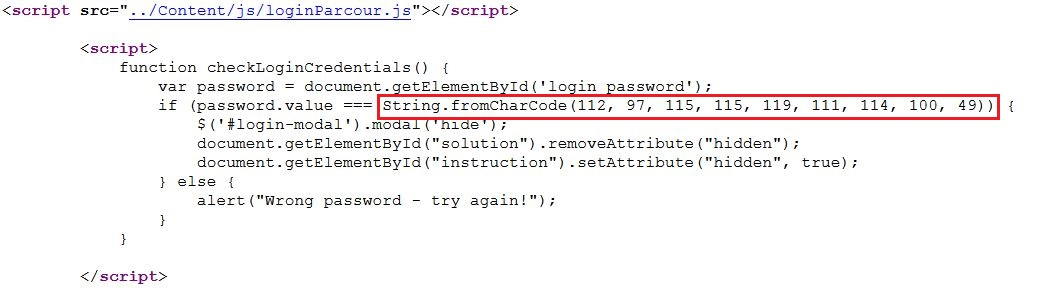
\includegraphics[width=\textwidth]{images/LoginParcours/login_level2_solution.jpg}
	\caption{Codeausschnitt zur Lösung des zweiten Levels}
	\label{fig:login-parcours-level2-solution}
\end{figure}

Erkenntlich wird dabei, dass das Passwort aus der Zahlenfolge\\ \colorbox{altgray}{\lstinline|112, 97, 115, 115, 119, 111, 114, 100, 49|} besteht. Übersetzt man diese nun in eine ASCII-Zeichenfolge entsteht das Wort \colorbox{altgray}{\lstinline|password1|}, dass die Lösung dieses Rätsels entspricht.

\subsection{Level 3 - Source Code Suche} 
Im folgenden Level muss der Anwender den Source Code zuerst finden, bevor er die Lösung herauslesen kann. Hierbei wurde in diesem Level der Rechtsklick mit der Maus deaktiviert. In der Praxis ist es jedoch nicht möglich den Source Code zu verstecken, da dieser auf der Clientseite und somit im Browser vorliegen muss. \\ 
Der Einsteiger muss folglich auf die Idee kommen, den Source Code mit der richtigen URL-Anfrage auszulesen. Die Lösung hierzu ist die Anweisung \colorbox{altgray}{\lstinline|view-source:http://|}. Die Abbildung \ref{fig:login-parcours-level3-solution} zeigt wiederum den relevanten Codeausschnitt mit dem Passwort.

\begin{figure}[H]
	\centering
	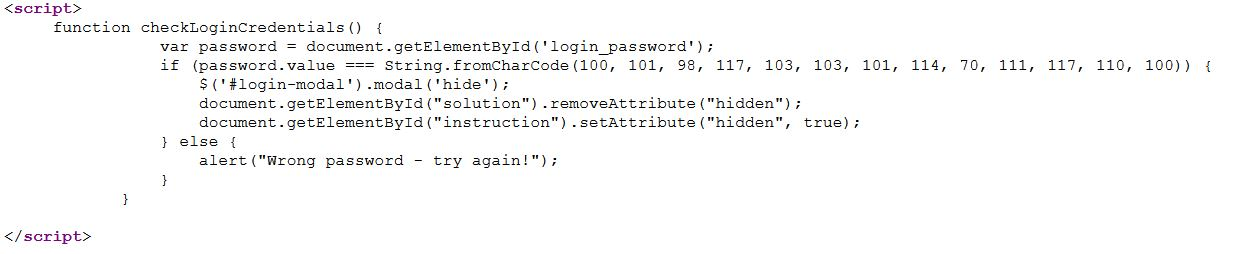
\includegraphics[width=\textwidth]{images/LoginParcours/login_level3_solution.jpg}
	\caption{Codeausschnitt zur Lösung des dritten Levels}
	\label{fig:login-parcours-level3-solution}
\end{figure}

Auch hier wurde eine Zahlenfolge gewählt, die in ASCII-Zeichen umgewandelt wird. So generiert sich das Passwort für dies Level aus der Zahlenfolge \colorbox{altgray}{\lstinline|100, 101, 98, 117, 103, 103, 101, 114, 70, 111, 117, 110, 100|} und entspricht  \colorbox{altgray}{\lstinline|debuggerFound|}. 

\subsection{Level 4 - Verstecke Dateien}
Im vierten Level ist eine Datei versteckt, die dem Einsteiger Hinweise zur Lösung des Rätsels gibt. Die Beschreibung des Rätsels ist wie folgt: \\
\textit{Bob ist kein guter Entwickler. Er hat das Passwort vergessen und murmelt die ganze Zeit nur etwas von aliens.txt. Ich weiß auch nicht was das bedeuten soll?!}
\\
Um das Rätsel zu lösen muss der Einsteiger, die Datei aliens.txt in der URL suchen. Abbildung \ref{fig:login-parcours-level4-hint} zeigt die gefundene Textdatei. 

\begin{figure}[H]
	\centering
	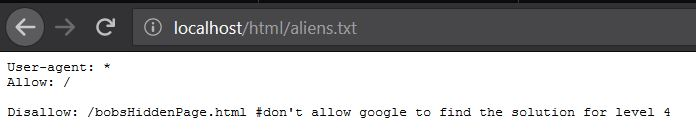
\includegraphics[width=\textwidth]{images/LoginParcours/login_level4_file.jpg}
	\caption{Gefundene Datei des vierten Levels}
	\label{fig:login-parcours-level4-hint}
\end{figure}

In dieser Textdatei wird auf eine versteckte Seite verwiesen, die in der gesamten Webanwendung durch keinen Link erreichbar ist. Die Abbildung \ref{fig:login-parcours-level4-solution} zeigt die versteckte Seite auf der das Passwort \colorbox{altgray}{\lstinline|bobIsSoStupid123|} ersichtlich ist. \\

\begin{figure}[H]
	\centering
	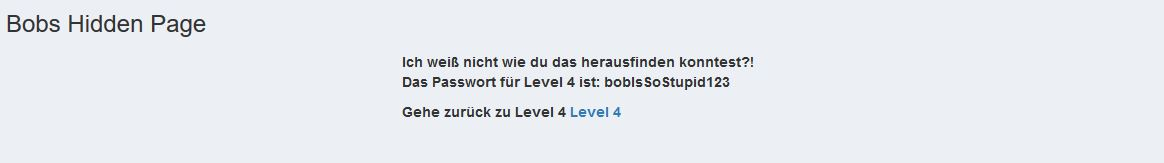
\includegraphics[width=\textwidth]{images/LoginParcours/login_level4_solution.jpg}
	\caption{Lösung des vierten Levels}
	\label{fig:login-parcours-level4-solution}
\end{figure} 

Abschließend muss in diesem Level erwähnt werden, dass die Validierung des Passworts nicht browserseitig geschieht, sondern mittels PHP auf dem Server. Folglich ist es dem Einsteiger nicht wie bisher möglich, dass Passwort im JavaScript Code wiederzufinden. 

\subsection{Level 5 - Caesar-Verschlüsselung}
Das fünfte Level umfasst eine Caesar-Verschlüsselung. Um folglich das Level zu lösen muss der Einsteiger wissen worum es sich bei dieser Verschlüsselung handelt. \\ 
\subsubsection*{Die Caesar-Verschlüsslung}
Gerade die Caesar-Verschlüsselung bietet sich als Einstiegs- und Demonstrationsverschlüsselung an, da mit ihr leicht die Grundlagen der Kryptographie gezeigt werden können. Allerdings ist das Verwenden der Caesar-Verschlüsselung nicht sehr sicher und kann leicht geknackt werden. Dieses Level des Login Parcours soll dies demonstrieren. \\ 
Prinzipiell ist die Caesar-Verschlüsslung ein einfaches symmetrisches Verschlüsselungsverfahren aus Zeiten der Römer und geht auf den Feldherr Julius Caesar zurück. \\
Konkret basiert die Caesar Chiffre auf einer monographischen und monoalphabetischen Substitution. Ausgangspunkt ist das Alphabet so wie wir es kennen. Nun wird jeder Buchstaben durch einen neuen Buchstaben ersetzt, nämlich der Buchstabe, der um drei Stellen versetzt ist. Aus einem "A" wird durch eine Verschiebung um drei Zeichen also der Buchstabe "D", ein "B" wird ein "E", das "C" ein "F" usw. Da das ganze zyklisch ist, wird das "X" durch ein "A" ersetzt, das "Y" durch ein "B" und das "Z" durch ein "C". Damit ergibt sich am Ende folgende Umwandlungstabelle (Siehe Abbildung \ref{fig:login-parcours-level5-caesar-theorie}):  

\begin{figure}[H]
	\centering
	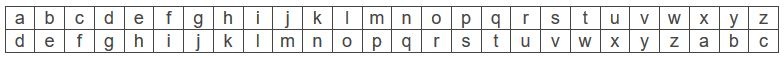
\includegraphics[width=\textwidth]{images/LoginParcours/login_parcrous_level5_caesar.jpg}
	\caption{Umsetzungstabelle bei der Caeser-Verschlüsselung mit Shift 3}
	\label{fig:login-parcours-level5-caesar-theorie}
\end{figure} 

Soll nun bspw. das Wort \textit{security} verschlüsseln, muss lediglich die obige Tabelle nach dem Buchstaben durchsucht werden und mit den dazugehörigen ersetzen. So entspricht \textit{security} in verschlüsselter Form \textit{vhfxulwb}. Zusätzlich kann der Verschiebungsfaktor des Alphabets beliebig gewählt werden, somit auch negativ. Zudem ist es bspw. möglich ein Wort mehrmals zu verschlüsseln. \\ 

\subsubsection*{Level 5}
In dem vorliegenden Passworträtsel bekommt der Einsteiger wieder eine Login-Maske (Siehe Abbildung \ref{fig:login-parcours-level5-caesar-maske}) vorgegeben mit dem Hinweis, dass das Passwort \textit{'LyRhtZhoBukZplnal'} lautet. Allerdings ist dieses mit der Caesar-Verschlüsselung encodiert worden.

\begin{figure}[H]
	\centering
	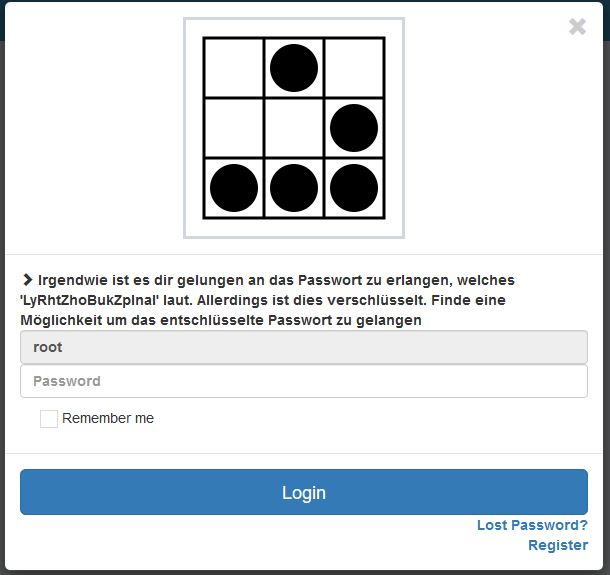
\includegraphics[width=\textwidth]{images/LoginParcours/login_parcrous_level5_caesar_maske.jpg}
	\caption{Login-Maske der Caesar-Verschlüsslung im fünften Level}
	\label{fig:login-parcours-level5-caesar-maske}
\end{figure} 

Um herauszufinden wie das decodierte Passwort aussieht muss der Einsteiger folglich die Verschiebung des Alphabets herausfinden. So könnte der Einsteiger z. B. ein eigenes Skript schreiben oder einen Caeser-Verschlüsslungsprogamm (https://gc.de/gc/caesar/) nutzen und jeden Verschiebungsfaktor durch zu spielen bis ein sinnvolles Passwort herauskommt. Bei dem Durchexerzieren sollte erkenntlich werden, dass bei einer Verschiebung um den Faktor -7, die Lösung für dieses Level herauskommt. Das korrekt entschlüsselte Passwort lautet \colorbox{altgray}{\lstinline|ErKamSahUndSiegte|}

\subsection{Level 6 - Wireshark-Sniffing}
Im sechsten Level des Parcours soll der Einsteiger in Kontakt mit Wireshark kommen. Die Abbildung \ref{fig:login_parcrous_level6_wireshark_maske} zeigt die Aufgabenstellung. 

\begin{figure}[H]
	\centering
	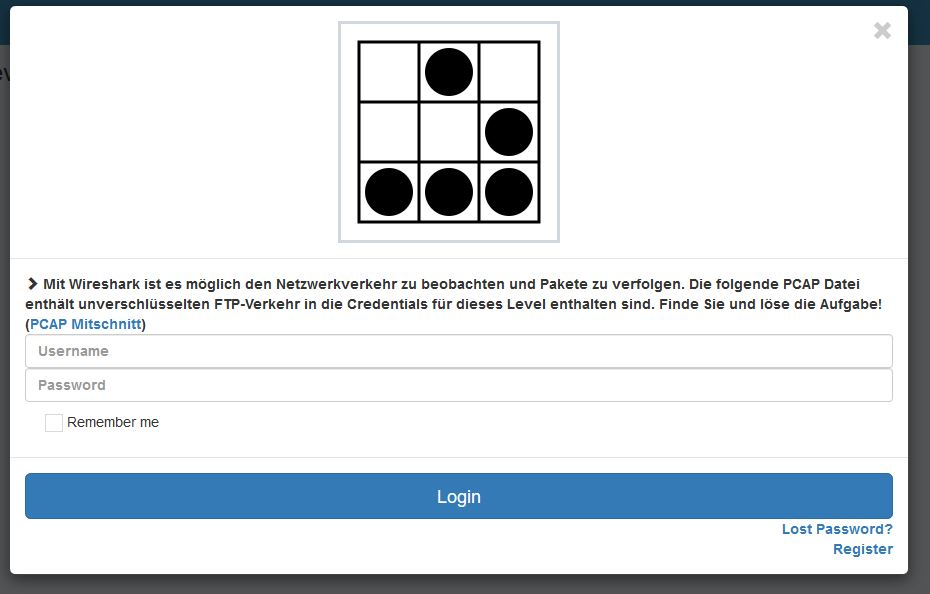
\includegraphics[width=\textwidth]{images/LoginParcours/login_parcrous_level6_wireshark_maske.jpg}
	\caption{Login-Maske des sechsten Levels}
	\label{fig:login_parcrous_level6_wireshark_maske}
\end{figure}

Hier soll der Einsteiger eine unverschlüsselte PCAP-Datei auslesen, die einen Nachrichtenverkehr wiedergibt. In dieser Datei ist an einer Stelle, der Username mit Passwort auslesbar. Abbildung \ref{fig:login_parcrous_level6_wireshark_solution} zeigt den relevanten Ausschnitt in Wireshark. Die Lösung des Levels ist der Username \colorbox{altgray}{\lstinline|jerry|} und das Passwort \colorbox{altgray}{\lstinline|saymynameheisenberg|}. 

\begin{figure}[H]
	\centering
	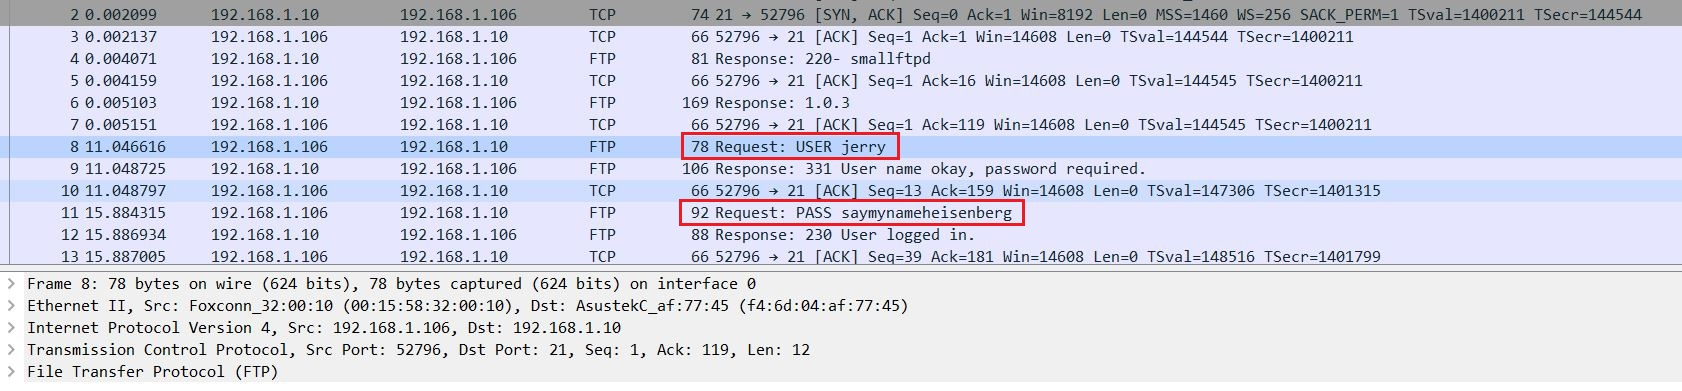
\includegraphics[width=\textwidth]{images/LoginParcours/login_parcrous_level6_wireshark_solution.jpg}
	\caption{Wiresharkausschnitt für die Lösung des sechsten Levels}
	\label{fig:login_parcrous_level6_wireshark_solution}
\end{figure}

\subsection{Level 7 - BCrypt-Verschlüsselung}
Das letzte Level umfasst einen weiteren Verschlüsselungsart - der BCrypt-Verschlüsselung. BCrypt ist eine kryptologische Hashfunktion, die speziell für das Hashen und Speichern von Passwörtern entwickelt wurde. Für dieses Level wurde die eingebaute BCrypt Funktion von PHP verwendet. \\
In der Aufgabe findet der Einsteiger eine Login-Maske (Siehe Abbildung \ref{fig:login_parcrous_level7_bcrypt_maske} wieder, in der eine Tabelle mit verschlüsselten Passwörtern enthalten ist. Zudem ist eine Liste von sogenannten \textit{Common-Passwords} gegeben, die häufig genutzte Passwörter wieder spiegelt. Somit ist die Aufgabe die gegebenen Passwörter zu entschlüsseln und zu überprüfen ob diese mit einem, der \textit{Common-Passwords} übereinstimmt. 

\begin{figure}[H]
	\centering
	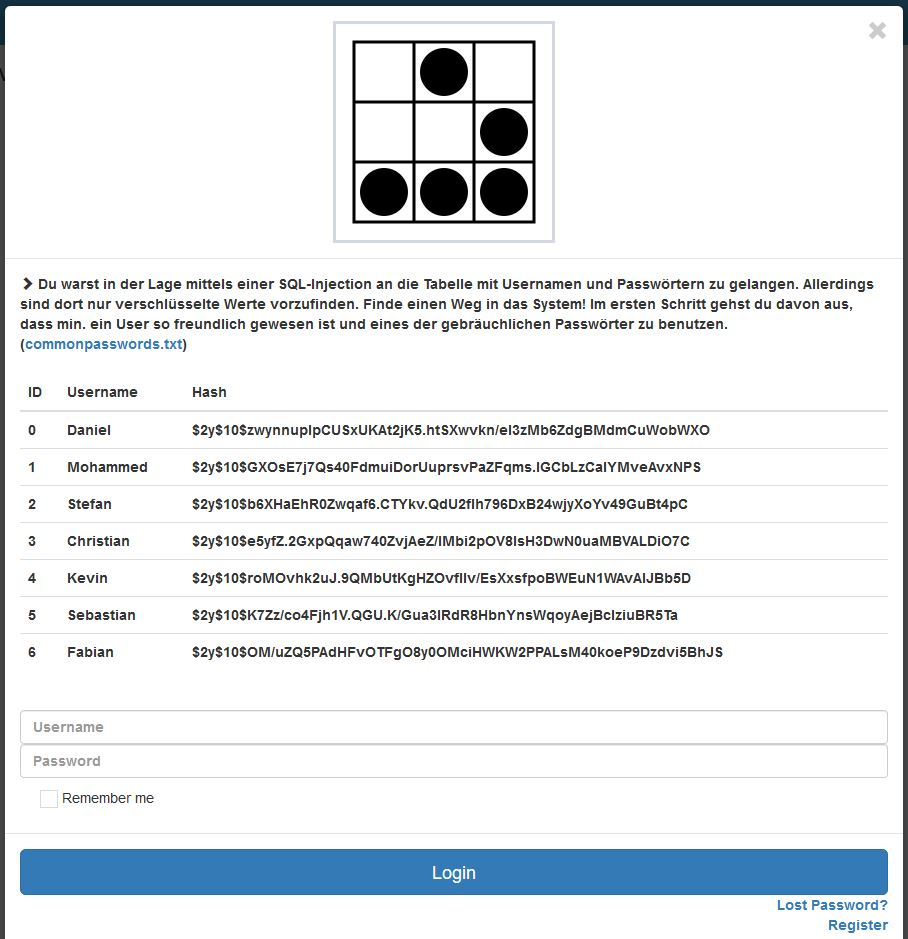
\includegraphics[width=\textwidth]{images/LoginParcours/login_parcrous_level7_bcrypt_maske.jpg}
	\caption{BCrypt Login Maske mit gegebenen Credentials}
	\label{fig:login_parcrous_level7_bcrypt_maske}
\end{figure}

Die Lösung für dieses Level lautet: Username \colorbox{altgray}{\lstinline|Kevin|} und Passwort \colorbox{altgray}{\lstinline|sniffing|}.

\section{Ausblick}
In Bezug auf die künftigen Entwicklungsschritte des Login Parcours sollen nun einige Vorschläge gemacht werden. \\ 
Die bisherigen Level orientieren sich zum Teil an Beispielübungen der Seite http://0xf.at/. Dort ist ein ähnliche Aufgabensammlung aufgezeigt, die als Inspiration gelten kann. Denkbar ist es auch, den Login Parcours in Richtung echter Hacker-Rätsel wie z. B. auf https://www.root-me.org/ aufzubauen. Diesbezüglich kann dies auch zusammen mit der Austragung des eigenen CTFs geschehen, der zum ersten Mal im Februar 2018 stattfindet.